
In the proposed architecture, the \textit{SmartBox} plays the role of acquiring the data that is transmitted wirelessly by the \textit{Biostickers}.
Each \textit{SmartBox} is associated to a single patient, it captures the data of each \textit{Biosticker} attached to that patient, and stores it in a local database for redundancy. 
It should also be capable of analyzing and process the data in real time, before propagating it to the higher layers in the system architecture, in order to reduce computation and networking overhead on the Smart Gateway. The \acs{WoW} project also foresees the usage of a classification algorithm in the \textit{SmartBox} to determine the body pose of the patient, as well as filtering the respiration data to account for signal fluctuations caused by sudden movements by the patient.  


\paragraph{} Additionally, for debugging purposes, researchers at the \acs{ISR} developed a simple developer \acs{GUI}, which can be seen on Figure \ref{fig:smartbox-gui}.

\begin{figure}[H]
    \centering
    \includegraphics[width=\linewidth]{images/smartbox-gui.png}
    \caption{Illustration of the developer \acf{GUI} for debugging the \textit{SmartBox} acquisition, designed by the \acs{WoW} research team at \acs{ISR}.}
    \label{fig:smartbox-gui}
\end{figure}

\paragraph{} Regarding data acquisition, the \textit{SmartBox} collects 5 distinct biosignals, which can be seen on the developer low level \acs{GUI} on Figure \ref{fig:smartbox-gui}:

\begin{itemize}
    \item \acf{ECG} -- Byte array (20 byte length) with the electrical signal measured, with a frequency of 20Hz.
    \item Respiration Rate -- An unsigned integer (4 bytes) representation of the rate of respiration, with a frequency of 10Hz.
    \item Heart Rate -- An unsigned byte representation of the heart rate in \textit{beats per minute}, every 5s.
    \item Body Temperature -- An IEEE 11073\footnote{\url{https://standards.ieee.org/standard/11073-10207-2017.html}} floating-point number representation of the body temperature, every 60s.
    \item Oxygen Saturation -- A standard floating-point number (4 bytes) representation of the oxygen saturation, with a frequency of 1Hz.
\end{itemize}

\todo[inline]{Todo: Confirm with @Bernardo acquisition rates for each value.}
\todo[inline]{Todo: Ask @Miguel for a picture of the biostickers.}
\section{Deciding on a Hardware Platform}

In the context of this dissertation, two different \acl{SBC}s (\acs{SBC}) were considered for the development of the \textit{SmartBox}: a Raspberry Pi 4 Model B and an UDOO BOLT v3. In the following sections we discuss and compare the characteristics of each platform. 

\subsubsection{Raspberry Pi 4 Model B}

Raspberry Pi denotes a series of \acs{SBC}s which are developed by the Raspberry Pi Foundation, a UK-based charity that aims to educate the general public about the power of computing and digital making, in association with Broadcom. It is one of the most popular hardware platforms used by developers due to its accessible price and community support \cite{jain2021introduction}.
At the time of the writing, the Raspberry Pi 4 Model B (or Raspberry Pi 4B)\footnote{\url{https://www.raspberrypi.com/products/raspberry-pi-4-model-b/}}, which can be seen in Figure \ref{fig:raspberrypi-image}, is the latest revision of the Raspberry Pi series, powered by Broadcom BCM2711 System on a Chip (SoC).

\begin{figure}[H]
    \centering
    \includegraphics[width=\linewidth]{images/raspberry-4-modele-b-4go.jpg}
    \caption{Raspberry Pi 4B.}
    \label{fig:raspberrypi-image}
\end{figure}

\subsubsection{UDOO BOLT V3}

As stated by the manufacturer\footnote{Product Website: https://www.udoo.org/discover-the-udoo-bolt/}, the ``UDOO BOLT is a quantum leap compared to current maker boards''. It represents a series of high performance \acs{SBC}, equipped with the latest generation of AMD Ryzen Embedded SoC. Additionally, it contains an Arduino Compatible microcontroller (connected via UART), making the UDOO BOLT extremely versatile.
The UDOO Bolt is incredibly well-supported by UDOO but unfortunately, it does not have nearly the same community support of Raspberry Pi.

\paragraph{} The UDOO BOLT V3, which can be seen in Figure \ref{fig:udoobolt-image}, is the entry-level product of the series, but it is still capable of allegedly outperforming full-fledged computers such as the Apple MacBook Pro 13", which just goes to show how powerful these \acs{SBC}s can be.

\todo[inline]{To-do: If time allows it, remake this with better quality.}

\begin{figure}[H]
    \centering
    \includegraphics[width=\linewidth]{images/UDOO_BOLT_GEAR_BLT.png}
    \caption{UDOO BOLT V3.}
    \label{fig:udoobolt-image}
\end{figure}

\subsection{Comparing the Hardware Platforms}

In order to decide on which platform to pick for the development of the project, it is crucial to compare the specification of both boards, which can be seen in the Table \ref{tab:comparsion-hardwareplatform}.

\renewcommand{\arraystretch}{2.5}
\begin{table}[H]
    \centering
    \begin{tabular}{r|l|l}
        %\textbf{Features} 
        & \textbf{Raspberry Pi 4B}& \textbf{UDOO BOLT V3}  \\ \hline
        \textbf{SoC} &  \makecell{Broadcom BCM2711 \\ (ARMv8 64-bit) \\ 4-core @ 1.5GHz} & \makecell{AMD Ryzen™ Embedded V1202B \\ (AMD64 64-bit) 2-core @ 2.3GHz \\ (up to 3.2GHz turbo)}\\
        \textbf{RAM} & 2, 4 or 8GB LPDDR4 & Up to 32GB DDR4 (Not included) \\ 
        \textbf{Storage} & \makecell{No internal storage, \\ SDXC Card Support} & \makecell{32GB internal eMMC + \\1 × SATA III and \\ 2 × M.2 connectors}\\
        \textbf{Networking} & \makecell{2.4/5.0 GHz WiFi, Gigabit \\ Ethernet, Bluetooth 5.0, BLE} & \makecell{Gigabit Ethernet + M.2 Key E slot \\ for optional WiFi+BT module}\\ 
        \textbf{I/O Ports} & \makecell{ 2 × USB 3.0, 2 × USB 2.0, \\ 2 × (Mini) HDMI} & \makecell{2 × USB 3.0 Type-A, \\ 2 × USB Type-C (w/ Display Port \\ + Power Delivery), 2 × HDMI} \\
        \makecell[r]{\textbf{Other} \\\textbf{Features}} & \makecell{Power over Ethernet \\(PoE)–enabled} & \makecell{Includes ATmega32U4 microcontroller\\ (Arduino Leonardo compatible), \\ RTC Battery} \\   
        \textbf{Dimensions} & 8.5 x 5.6 x 1.7 cm & 12 x 12 x 7 cm \\
        \textbf{Price} & \makecell{75.93 € (\textbf{8GB Model}, \\ including a 32GB SDXC Card\\ and case)} & \makecell{534.48 € (including external power \\ supply and a 16GB RAM module)} \\
    \end{tabular}
    \caption{Specifications of the Raspberry Pi 4B and UDOO BOLT V3.}
    \label{tab:comparsion-hardwareplatform}
\end{table}
\renewcommand{\arraystretch}{1}


\paragraph{} From the Table \ref{tab:comparsion-hardwareplatform}, we immediately conclude that the Raspberry Pi is a much more affordable alternative. At over 1/7 of the price, it already has a working WiFi+BT networking module (which is not included in the UDOO BOLT), nearly identical Input/Output (I/O) port capability and a smaller size. UDOO BOLT V3 on the other hand, has a much better SoC, which is expected to delivery a much better overall computing performance.


\paragraph{} In order to understand how these differences in the hardware specification between the \acs{SBC}s translate to real-world performance, a test suite was developed and conducted to quantify the performance of each \acs{SBC}. The tools developed for each test can be found here\footnote{\url{https://github.com/WoW-Institute-of-Systems-and-Robotics/smartbox\_benchmark\_tests}}. 

\paragraph{}Below, we detail how each test works and discuss how each \acs{SBC} performed. 

\subsubsection{Test 1: Python Benchmark}

Given the data processing requirements for the \textit{SmartBox}, and as Python will be used as the main scripting language for most of the \textit{SmartBox} development, we developed a simple test to estimate computing performance, or more specifically (single-threaded) performance of arithmetic tasks, on each \acs{SBC}. In this test, each \acs{SBC} calculates the \textit{n}-th number in the Fibonacci sequence \cite{pierce1951fibonacci}, and we measure the time taken. This process is repeated 10 times for different numbers, from 10000 to 500000, to determine average run time.

\begin{figure}[H]
    \centering
    \includegraphics[width=0.8 \linewidth]{images/fibonacci-test.pdf}
    \caption [Custom Python benchmark for the Raspberry Pi 4B and UDOO BOLT V3.]{ Custom Python benchmark for the Raspberry Pi 4B and UDOO BOLT V3. The standard deviation for each run time is inferior to 0.1\% in each test, and therefore it is not displayed in the figure.}
    \label{fig:fibonacci-tests}
\end{figure}

From Figure \ref{fig:fibonacci-tests}, we can observe that the time taken for computing each number increases exponentially for each platform. By analyzing the data, we can see that the UDOO BOLT V3 outperforms Raspberry Pi 4B on average by a factor of 2.5 $\pm$ 0.2.

\subsubsection{Test 2: Phoronix Test Suite}

The Phoronix Test Suite\footnote{Phoronix Test Suite - Linux Testing \& Benchmarking Platform, Automated Testing, Open-Source Benchmarking: \url{https://www.phoronix-test-suite.com/}} is an open-source benchmarking platform used for comparing the performance of different systems. The framework provides compilations of tests for a variety of tools and is also fully customizable and expandable, allowing users to develop and automate their own tests in a clean, reproducible and easy-to-use fashion. The test profiles work by measuring some property of the benchmark, (\textit{e.g.} the run time for calculating the first 100 Fibonacci numbers) and use it to provide an estimate of the performance of the \acs{SBC}, which can be easily used for comparison between different systems. 

\paragraph{} For the purposes of evaluating the computing performance of each \acs{SBC}, we chose the following standard test profiles provided by Phoronix\footnote{OpenBenchmarking.org - Cross-Platform, Open-Source Automated Benchmarking Platform: \url{https://openbenchmarking.org/}}, which are a compilation of the most popular Python and CPU benchmarks used:

\begin{itemize}
    \item BYTE Unix Benchmark (``BYTE''), single-threaded CPU benchmark -- Runs BYTE UNIX benchmark suite (more particularly, the Dhrystone 2 synthetic benchmark) to measure the amount of instructions per second (IPS). 
    \item 7-Zip Compression (``7-Zip''), multithreaded CPU benchmark -- Runs the benchmark feature integrated in 7-Zip to measure the amount of millions instructions per second (MIPS). The benchmark consists of a LZMA data compression and decompression test run, using all available threads in the system (meaning it will scale highly with the amount of threads in the system). 
    \item PyBench Benchmark (``PyBench''), single-threaded Python \& CPU benchmark -- Executes different function such as built-in function calls and nested for-loops and measures its runtime.
    \item PyPerformance \textit{chaos} Benchmark (``chaos''), single-threaded Python \& CPU benchmark -- Create chaos game-like fractals \cite{Jeffrey1992} and measures its run-time. 
    \item PyPerformance \textit{float} Benchmark (``float''), single-threaded Python \& CPU benchmark -- Create 100,000 random floating-point numbers and calculate the co-sine, sine and square root of each one and measures its run-time.
    \item PyPerformance \textit{nbody} Benchmark (``nbody''), single-threaded Python \& CPU benchmark -- Runs an \textit{n-body} problem simulation \cite{Playne2009} and measures its run-time.
    \item PyPerformance \textit{json\_loads} Benchmark (``json''), single-threaded Python \& CPU benchmark -- Evaluates \acf{JSON}\footnote{The JavaScript Object Notation (JSON) Data Interchange Format: \url{https://www.rfc-editor.org/rfc/rfc8259.html}} parsing and serialization, a widely used open stardard data format, by dumping and loading thousands of objects and measures its runtime.
    \item PyPerformance \textit{crypto\_pyaes} Benchmark (``crypto''), single-threaded Python \& CPU benchmark -- Runs the AES block-cipher Python implementation and measures its run-time.
    \item PyPerformance \textit{regex\_compile} Benchmark (``regex''), single-threaded Python \& CPU benchmark -- Compiles different \textit{regular expressions} or \textit{regexes} in Python and measures its run-time.
    \item PyPerformance \textit{python\_startup} Benchmark (``startup''), single-threaded Python \& general system perforamnce benchmark -- Measures Python's startup time.
    \item PyPerformance \textit{django\_template} Benchmark (``django''), single-threaded Python benchmark -- Builds a 150x150-cell HTML table and measures its run-time.
\end{itemize}

\paragraph{} The benchmark results obtained were published to the \textit{OpenBenchmarking.org} website, and can be found by visiting the following webpage: \url{https://openbenchmarking.org/result/2110255-JNCF-211025851}.
\begin{figure}[H]
    \centering
    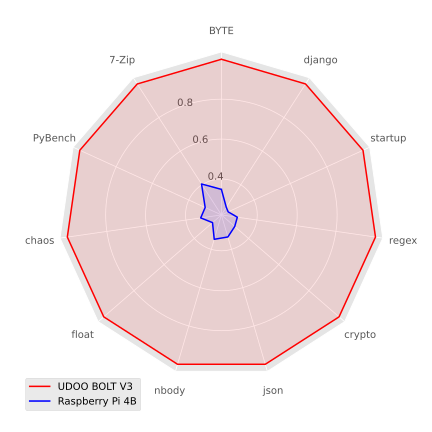
\includegraphics[width=0.8 \linewidth]{images/phoronix-benchmarks.pdf}
    \caption [Phoronix benchmarks results for the UDOO BOLT V3 and Raspberry Pi 4B.]{ Phoronix benchmarks results for the UDOO BOLT V3 and Raspberry Pi 4B. The performance values for each test are normalized to UDOO BOLT V3 performance.}
    \label{fig:phronix-benchmarks}
\end{figure}

\paragraph{} From the Figure \ref{fig:phronix-benchmarks}, we can observe that UDOO BOLT V3 performs much better than Raspberry Pi 4B in every benchmark, as expected. By analyzing the data, we find that UDOO BOLT V3 outperforms Raspberry Pi 4B on average by a factor of 2.21 $\pm$ 0.4.

\subsubsection{Test 3: \acs{MQTT} Benchmark}

As the \textit{SmartBox} will communicate with the Smart Gateway through \acs{MQTT}, we decided to evaluate how each system handles the load associated with an \acs{MQTT} client. For this test, each \acs{SBC} ran a simple \acs{MQTT} client which was subscribing to a single topic and publishing to another topic using a given transmission rate, a message with a payload containing the string ``hello world'' to a \acs{MQTT} broker in the local network.

\begin{figure}[H]
    \centering
    \includegraphics[width=\linewidth]{images/mqtt_test_results.pdf}
    \caption[Results of the \acs{MQTT} benchmark for Raspberry Pi 4B and UDOO BOLT V3.]{Results of the \acs{MQTT} benchmark for Raspberry Pi 4B and UDOO BOLT V3. As the transmission frequency increases, we observe that the Raspberry Pi consumes more resources than the UDOO BOLT V3, nonetheless, these are very negligible performance differences, with an impact of < 0.5\% resource usage.}
    \label{fig:mqtt-tests}
\end{figure}

The \acs{MQTT} client is a very lightweight process, and as seen in Figure \ref{fig:mqtt-tests}, is capable of running on both platforms with trivial performance impact.

\subsubsection{Conclusion}

Based on the results of our tests we conclude that UDOO BOLT V3 heavily outperforms the Raspberry Pi 4B in CPU benchmarks, but shows a negligible difference in memory usage. Nonetheless, we find that these performance gains do not meaningfully impact the \textit{SmartBox} functionality, for example, in the \acs{MQTT} communication. Due to the extremely affordable price of the Raspberry Pi 4B, we have decided to move forward with the Raspberry Pi 4B for the development of the project.

\clearpage

\section{Communication with the Biostickers}

As previously mentioned, the communication between the \textit{Biostickers} and the \textit{SmartBox} makes use of the \acs{BLE} protocol. One of the advantages of using the Raspberry Pi 4B, as discussed in the previous section, is the fact that it already includes all networking functionality needed for the project. 

\paragraph{} However, the communication with the \textit{Biostickers} is very critical and demanding. During the development of the project, the research team has decided to use a \textit{Biosticker} coupled with a commercially available Pulse Oximeter in order to capture all required biosignals. This means that the \acs{BLE} acquisition system must be capable of handling both communications simultaneously. Having this in mind, we need to understand if the included \acs{BLE} adapter of the Raspberry Pi board is sufficient for the task, or if we need to consider a different acquisition hardware.

\paragraph{} In order to understand how data transmission works between \acs{BLE} devices, some technical background regarding the data transmission in protocol is presented.

\subsection{Technical Background} 
 % Ver https://www.scirp.org/journal/paperinformation.aspx?paperid=103686

% \todo[inline]{To-do: Intro to Link Layer, LE 1M e 2M, packet format, mention GATT and overview data transmission...}

The \acs{BLE} protocol stack is organized into three major components, as shown in Figure \ref{fig:ble-protocol-stack}: the Application Layer, the Host Layer and Controller Layer. 

\begin{figure}[H]
    \centering
    \includegraphics[width=0.6\linewidth]{images/ble protocol stack.pdf}
    \caption[Diagram of the different components of the \acs{BLE} protocol stack.]{Diagram of the different components of the \acs{BLE} protocol stack. Adapted from \cite{Specification1999, Farej2020}}
    \label{fig:ble-protocol-stack}
\end{figure}

At the Controller layer, we have the \acf{PHY} and \acf{LL} components.

The \acf{PHY} is the bottom layer of the \acs{BLE} stack, and is responsible for the transmission and reception of information over radio waves on the Industrial Scientific Medical (ISM) 2.4GHz band.

The Host Layer contains the higher level protocols of the protocol stack that interact with the application level layers. 

The \acs{L2CAP} is responsible for encapsulates the data from the higher layers in the protocol stack and


, such as \acf{L2CAP}, \acf{GAP},  while the Controller Layer handles the lower layers related to 

The Application Layer contains the user application, which interfaces with the Bluetooth protocol stack.

The data packet format for \acs{BLE} messages is shown in Figure \ref{fig:ble-ll-packet-format}.

The \acs{L2CAP} is responsible for encapsulates the data from the higher layers in the protocol stack and


The L2CAP achieves the transmission of the large data packets by segmenting and then at the receiver, re-assembling the packets so that the data can be fitted into the limits of the lower layer data packets.

\begin{figure}[H]
    \centering
    \includegraphics[width=\linewidth]{images/bluetooth data packet format.pdf}
    \caption[Diagram of the \acs{BLE} data packet format for uncoded \acs{PHY}s (LE 1M and LE 2M).]{\acs{BLE} data packet format for uncoded \acs{PHY}s (LE 1M and LE 2M). Adapted from \cite{Specification1999, Farej2020}.}
    \label{fig:ble-ll-packet-format}
\end{figure}


\paragraph{} Before we disuss \acs{BLE} data transmissions, it is important to indicate certain terminology which is used in the area:

\begin{itemize}
    \item Slave Latency: Number of consecutive connection events the slave device is not required to listen for the master. It allows a device to use a reduced number of connection events, thus minimizing power consumption.
\end{itemize}



\begin{itemize}
    \item Slave Latency: Number of consecutive connection events the slave device is not required to listen for the master. It allows a device to use a reduced number of connection events, thus minimizing power consumption.
    \item Connection Interval: Time between two consecutive connection events.
    \item Supervisor Timeout: Maximum time between two received data \acs{PDU}s before the connection is considered lost.
    \item \acf{MTU} for the \acs{ATT} protocol: Length of the \acs{PDU} for the \acs{ATT} protocol, which includes the \acs{ATT} header as well as the payload containing the data to be transmitted.
\end{itemize}


\begin{figure}[H]
    \centering
    \includegraphics[width=\linewidth]{images/ble-sending-data.pdf}
    \caption[Message sequence chart between two \acs{BLE} devices sending data and replying to the request.]{Message sequence chart between two \acs{BLE} devices sending data and replying to the request. Source: \cite{Specification1999}}
    \label{fig:ble-message-sequence-chart}
\end{figure}


\clearpage

\subsubsection{\acs{BLE} protocol stack on Linux} 

In the \acs{WoW} project, the data acquisition is developed using the official Linux implementation of \acs{BLE} protocol stack\footnote{\textit{BlueZ}: \url{http://www.bluez.org/profiles/}} -- \textit{BlueZ} -- in order to promote interoperability; since these drivers are developed and used by the community, allowing us to use multiple \acs{BLE} adapters, and even different \acs{SBC}s, using the same codebase without being tied down to proprietary code. 

\paragraph{} Currently, \textit{BlueZ} only officially supports up to the Bluetooth 4.2 specification, which is, at the time of writing, is still the predominantly used version \cite{Faria2020}. Nonetheless, Bluetooth specifications are generally backwards compatible with older versions.

\todo[inline]{Nota para @David Portugal: Isto é o que está indicado no website, mas existem funcionalidades de Bluetooth 5.X que estão implementadas (mas não especificam o escopo que está implementado). Indico alguma coisa sobre isso? Removo este parágrafo? Ou deixo tudo como está? }


\subsection{Choosing a \acs{BLE} adapter} 

\paragraph{} As mentioned previously, one of the objectives of this dissertation work is to analyze if the internal \acs{BLE} adapter provided by the Raspberry Pi 4B is sufficient for the \acs{WoW} project. To achieve this, we decided to compare this adapter with a commercially available that met the requirements for the project. The requirements for the adapter are the following:

\begin{itemize}
    \item The adapter must support, at least, the Bluetooth 5.0 core specification.
    \item The adapter must natively support Ubuntu 20.04, as well as the \textit{BlueZ} \acs{BLE} protocol stack. 
    %\item The adapter should support the LE 2M physical layer for better throughput.
\end{itemize}

\paragraph{} After researching the available market, we chose the Asus USB-BT500 USB adapter\footnote{Asus USB-BT500 Bluetooth 5.0 USB Adapter: \url{https://www.asus.com/Networking-IoT-Servers/Adapters/All-series/USB-BT500/}} due to its affordability and availability, making it an adequate fit for the project's needs.

\paragraph{} In the next section, we perform multiple tests to evaluate the performance of Asus USB-BT500 and the internal \acs{BLE} adapter in the Raspberry Pi 4B.

\subsection{Testing \acs{BLE} Communication} 

To ensure an \acs{BLE} adapter is capable of handling the communication on the \textit{SmartBox} side for the \acs{WoW} project, we created two different tests to evaluate their performance at different distances: a test to evaluate the roundtrip time for a single message (for different sizes), and a test to evaluate the maximum bandwidth achieveable using a packet loss analysis for multiple frequencies.


\subsubsection{Firmware developed for the tests}

In the \acs{WoW} project, 

\subsubsection{Test Conditions}

In order to ensure replicability and reliability of the test results, we use the same connection parameters for all tests, which are the following:

\begin{table}[H]
    \centering
    \begin{tabular}{|l|l|}
    \hline
    \textbf{Connection Interval} & 7.5ms \\ \hline
    \textbf{Slave Latency}       & 0     \\ \hline
    \textbf{Supervisor Timeout}  & 500ms \\ \hline
    \textbf{\acs{ATT} \acs{MTU} Length}      & 23 bytes   \\ \hline
    \end{tabular}
    \caption{\acs{BLE} connection parameters used for the ASUS USB-BT500 adapter.}
    \label{tab:ble-connection-values-hci1}
\end{table}

\begin{table}[H]
    \centering
    \begin{tabular}{|l|l|}
    \hline
    \textbf{Connection Interval} & 7.5ms \\ \hline
    \textbf{Slave Latency}       & 0     \\ \hline
    \textbf{Supervisor Timeout}  & 500ms \\ \hline
    \textbf{\acs{ATT} \acs{MTU} Length}      & 251 bytes   \\ \hline
    \end{tabular}
    \caption{\acs{BLE} connection parameters used for internal Raspberry Pi 4B adapter.}
    \label{tab:ble-connection-values-hci0}
\end{table}

Additionally, these tests were conducted indoors, with the devices (the \acs{BLE} adapter and the microcontroller) in clear view of each other.

\subsubsection{Test 1: Roundtrip Time Measurement}

In this first test, we measure the roundtrip time of a single \acs{ATT} data packet on a \acs{BLE} connection. 

\begin{figure}[H]
    \centering
    \includegraphics[width=0.75\linewidth]{images/ble-roundtrip-hci0-0cm.pdf}
    \label{fig:ble-roundtrip-hci0-0m}
    \caption[Average \acs{BLE} connection roundtrip time obtained for different distances using the Asus USB-BT500 adapter.]{Average \acs{BLE} connection roundtrip time obtained for different distances using the Asus USB-BT500 adapter.}
\end{figure}

\begin{figure}[H]
    \centering
    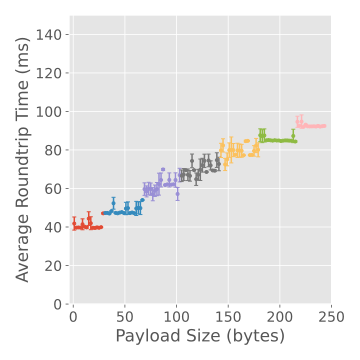
\includegraphics[width=0.75\linewidth]{images/ble-roundtrip-hci0-300cm.pdf}
    \label{fig:ble-roundtrip-hci0-3m}
    \caption[Average \acs{BLE} connection roundtrip time obtained for different distances using the Asus USB-BT500 adapter.]{Average \acs{BLE} connection roundtrip time obtained for different distances using the Asus USB-BT500 adapter.}
\end{figure}

\begin{figure}[H]
    \centering
    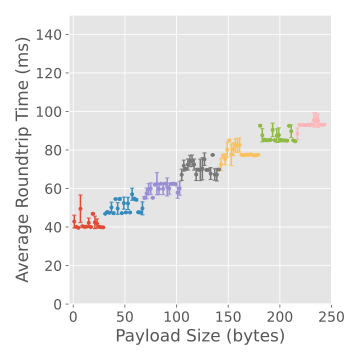
\includegraphics[width=0.75\linewidth]{images/ble-roundtrip-hci0-600cm.pdf}
    \label{fig:ble-roundtrip-hci0-6m}
    \caption[Average \acs{BLE} connection roundtrip time obtained for different distances using the Asus USB-BT500 adapter.]{Average \acs{BLE} connection roundtrip time obtained for different distances using the Asus USB-BT500 adapter.}
\end{figure}

\begin{figure}[H]
    \centering
    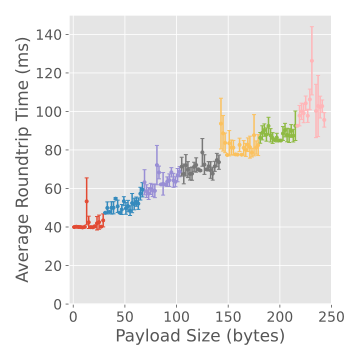
\includegraphics[width=0.75\linewidth]{images/ble-roundtrip-hci0-900cm.pdf}
    \label{fig:ble-roundtrip-hci0-9m}
    \caption[Average \acs{BLE} connection roundtrip time obtained for different distances using the Asus USB-BT500 adapter.]{Average \acs{BLE} connection roundtrip time obtained for different distances using the Asus USB-BT500 adapter.}
\end{figure}


\begin{figure}[H]
    \centering
    \includegraphics[width=0.75\linewidth]{images/ble-roundtrip-hci1-0cm.pdf}
    \label{fig:ble-roundtrip-hci1-0m}
    \caption[Average \acs{BLE} connection roundtrip time obtained for different distances using the Asus USB-BT500 adapter.]{Average \acs{BLE} connection roundtrip time obtained for different distances using the Asus USB-BT500 adapter.}
\end{figure}

\begin{figure}[H]
    \centering
    \includegraphics[width=0.75\linewidth]{images/ble-roundtrip-hci1-300cm.pdf}
    \label{fig:ble-roundtrip-hci1-3m}
    \caption[Average \acs{BLE} connection roundtrip time obtained for different distances using the Raspberry Pi 4B adapter.]{Average \acs{BLE} connection roundtrip time obtained for different distances using the Asus USB-BT500 adapter.}
\end{figure}

\begin{figure}[H]
    \centering
    \includegraphics[width=0.75\linewidth]{images/ble-roundtrip-hci1-600cm.pdf}
    \label{fig:ble-roundtrip-hci1-6m}
    \caption[Average \acs{BLE} connection roundtrip time obtained for different distances using the Asus USB-BT500 adapter.]{Average \acs{BLE} connection roundtrip time obtained for different distances using the Asus USB-BT500 adapter.}
\end{figure}

\begin{figure}[H]
    \centering
    \includegraphics[width=0.75\linewidth]{images/ble-roundtrip-hci1-900cm.pdf}
    \label{fig:ble-roundtrip-hci1-9m}
    \caption[Average \acs{BLE} connection roundtrip time obtained for different distances using the Asus USB-BT500 adapter.]{Average \acs{BLE} connection roundtrip time obtained for different distances using the Asus USB-BT500 adapter.}
\end{figure}



\subsubsection{Test 2: Bandwidth Measurement}
\todo[inline]{...}

\begin{figure}[H]
    \centering
    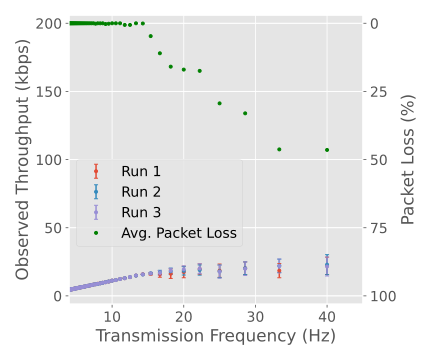
\includegraphics[width=0.75\linewidth]{images/ble-bandwidth-hci1-0cm.pdf}
    \label{fig:ble-bandwidth-hci1-0m}
    \caption[Average roundtrip time obtained at a distance of 9m using \acs{BLE} connection.]{Average \acs{BLE} connection roundtrip time at a distance of $9\text{m} \pm 0.2$.}
\end{figure}

\begin{figure}[H]
    \centering
    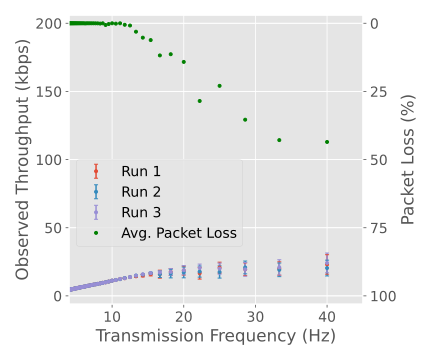
\includegraphics[width=0.75\linewidth]{images/ble-bandwidth-hci1-300cm.pdf}
    \label{fig:ble-bandwidth-hci1-3m}
    \caption[Average roundtrip time obtained at a distance of 9m using \acs{BLE} connection.]{Average \acs{BLE} connection roundtrip time at a distance of $9\text{m} \pm 0.2$.}
\end{figure}

\begin{figure}[H]
    \centering
    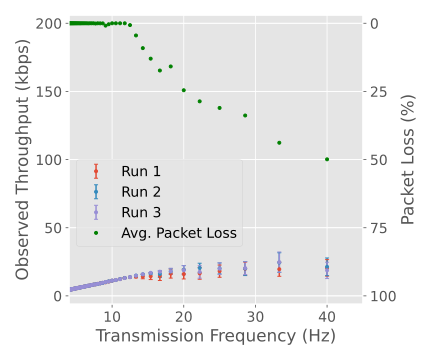
\includegraphics[width=0.75\linewidth]{images/ble-bandwidth-hci1-600cm.pdf}
    \label{fig:ble-bandwidth-hci1-6m}
    \caption[Average roundtrip time obtained at a distance of 9m using \acs{BLE} connection.]{Average \acs{BLE} connection roundtrip time at a distance of $9\text{m} \pm 0.2$.}
\end{figure}

\begin{figure}[H]
    \centering
    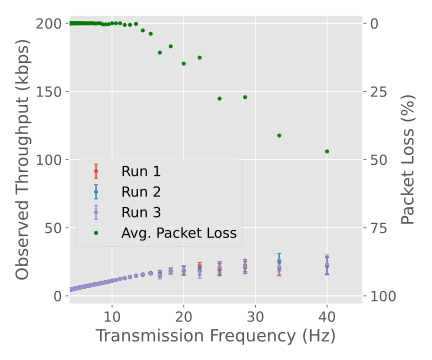
\includegraphics[width=0.75\linewidth]{images/ble-bandwidth-hci1-900cm.pdf}
    \label{fig:ble-bandwidth-hci1-9m}
    \caption[Average roundtrip time obtained at a distance of 9m using \acs{BLE} connection.]{Average \acs{BLE} connection roundtrip time at a distance of $9\text{m} \pm 0.2$.}
\end{figure}

\begin{figure}[H]
    \centering
    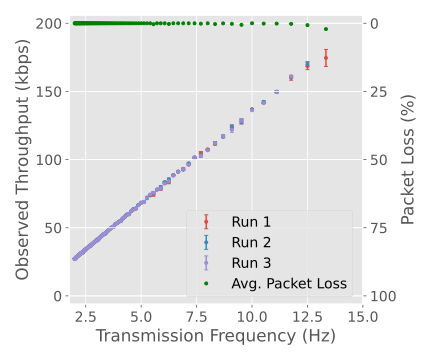
\includegraphics[width=0.75\linewidth]{images/ble-bandwidth-hci0-0cm.pdf}
    \label{fig:ble-bandwidth-hci0-0m}
    \caption[Average roundtrip time obtained at a distance of 9m using \acs{BLE} connection.]{Average \acs{BLE} connection roundtrip time at a distance of $9\text{m} \pm 0.2$.}
\end{figure}

\begin{figure}[H]
    \centering
    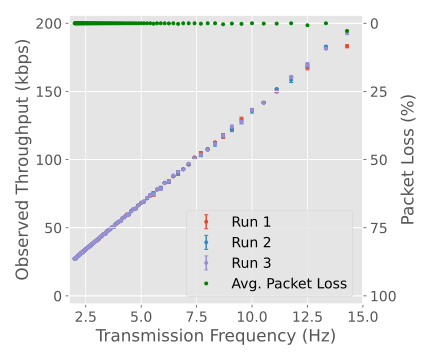
\includegraphics[width=0.75\linewidth]{images/ble-bandwidth-hci0-300cm.pdf}
    \label{fig:ble-bandwidth-hci0-3m}
    \caption[Average roundtrip time obtained at a distance of 9m using \acs{BLE} connection.]{Average \acs{BLE} connection roundtrip time at a distance of $9\text{m} \pm 0.2$.}
\end{figure}

\begin{figure}[H]
    \centering
    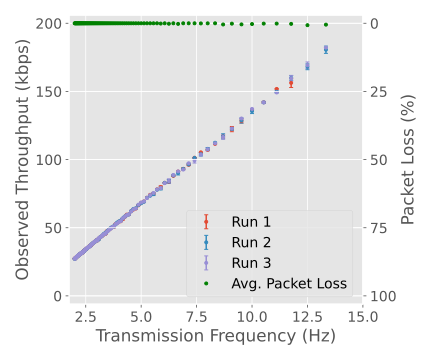
\includegraphics[width=0.75\linewidth]{images/ble-bandwidth-hci0-600cm.pdf}
    \label{fig:ble-bandwidth-hci0-6m}
    \caption[Average roundtrip time obtained at a distance of 9m using \acs{BLE} connection.]{Average \acs{BLE} connection roundtrip time at a distance of $9\text{m} \pm 0.2$.}
\end{figure}

\begin{figure}[H]
    \centering
    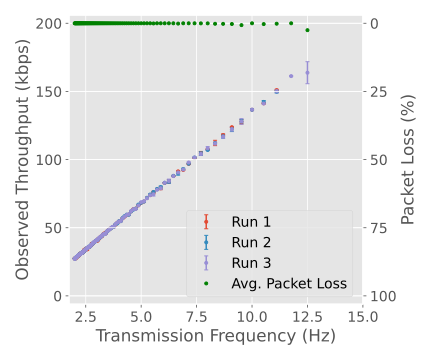
\includegraphics[width=0.75\linewidth]{images/ble-bandwidth-hci0-900cm.pdf}
    \label{fig:ble-bandwidth-hci0-9m}
    \caption[Average roundtrip time obtained at a distance of 9m using \acs{BLE} connection.]{Average \acs{BLE} connection roundtrip time at a distance of $9\text{m} \pm 0.2$.}
\end{figure}



\subsection{Decision on \acs{BLE} adapter}

\section{Summary}
In this chapter, we \dots